\documentclass{ximera}

\addPrintStyle{..}

\begin{document}
	\author{Bart Lambregs}
	\xmtitle{Arbeid geleverd door een niet-constante kracht}{}
    \xmsource\xmuitleg





	%%%\section{Arbeid van een niet-constante kracht}

	Algemeen zal een kracht gedurende de verplaatsing niet constant blijven. Ze zal met andere woorden o.a. afhankelijk zijn van de plaats waar het lichaam zich bevindt. We kunnen die afhankelijkheid beschrijven met behulp van een functie, de (grootte van de) kracht
	als functie van de plaats:
	\begin{eqnarray*}
	F&=&F(x)
	\end{eqnarray*}
	Eenvoudigheidshalve beperken we ons hier tot bewegingen op een rechte. Bewegingen in meerdere dimensies vereisen een uitgebreidere integraaltheorie dan hetgeen we nu kennen.
	
	We geven een opbouw om tot een definitie van arbeid te komen in het geval dat de kracht dus niet constant is. Ze vertoont gelijkenissen met de opbouw van de integraal.
	\begin{image}
	
	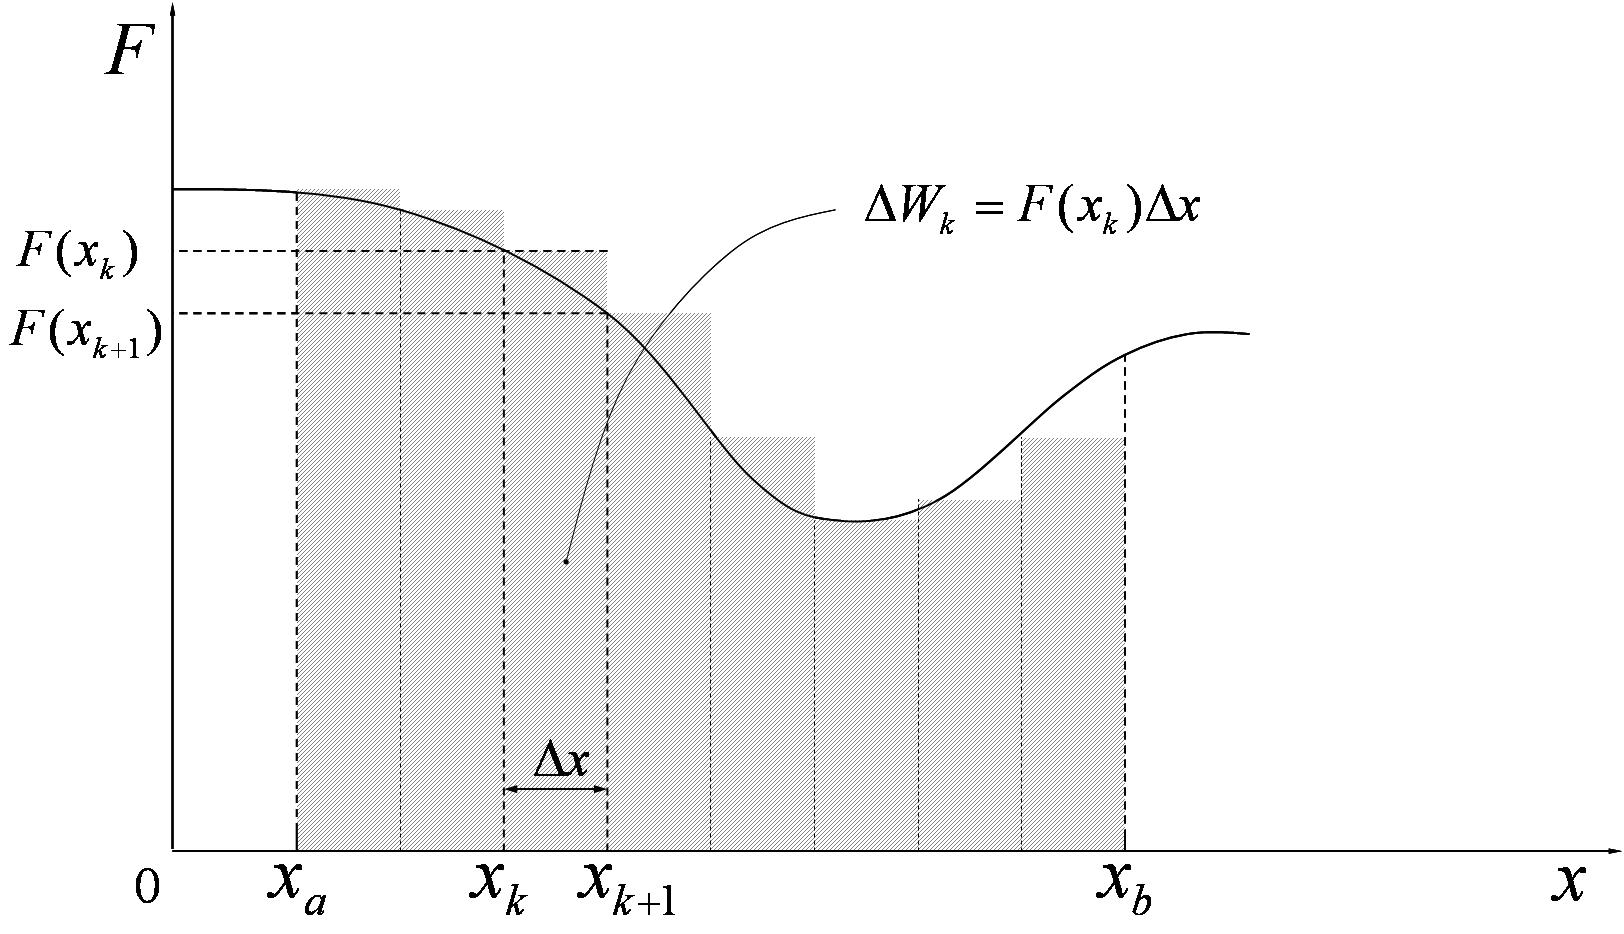
\includegraphics[width=0.85\textwidth]{arbeid_nietconstantekracht}
	\end{image}
	\captionof{figure}{Opbouw arbeid bij een niet-constante kracht}
	
	Verdeel de verplaatsing $x_b-x_a$ in heel veel hele kleine stukjes $\Delta x$ bijvoorbeeld als volgt:
	\begin{eqnarray*}
	\Delta x&=&\frac{x_b-x_a}{n}
	\end{eqnarray*}
	met $n\in\mathbb{N}_0$ zeer groot. De posities tussen de stukjes kunnen we dan be\-schrij\-ven door
	\begin{eqnarray*}
	x_k=x_a+k\Delta x\ \ k\in\{0,1,2,\ldots,n\}
	\end{eqnarray*}
	Hoe kleiner $\Delta x$ is, hoe minder de kracht binnen deze stukjes variëert en hoe meer dus $F(x_k)$ de kracht weergeeft die aanwezig is bij de verplaatsing van $x_{k}$ naar $x_{k+1}$. Het kleine stukje arbeid $\Delta W_k=F(x_k)\Delta x$ zouden we kunnen beschouwen als
	een benadering van de geleverde arbeid gedurende deze kleine verplaatsing. De arbeid geleverd bij de gehele verplaatsing zou dan overeen kunnen komen met de som van alle stukjes geleverde arbeid. Hoe kleiner we $\Delta x$ nemen hoe meer die som overeenkomt met wat de totale arbeid zou moeten zijn, vandaar dat in de limiet van $\Delta x$ gaande naar nul, we de geleverde arbeid zouden kunnen vinden. Deze limiet komt overeen met het nemen van een integraal:
	\begin{eqnarray*}
	W\,=\,\lim_{\Delta x\rightarrow0}\sum_{k=0}^{n-1}\Delta W_k
	%&=&\lim_{n\rightarrow\infty}\sum_{k=0}^{n-1}F(x_k)\Delta x\\
	\,=\,\lim_{n\rightarrow\infty}\sum_{k=0}^{n}F(x_k)\Delta x
	\,=\,\int_{x_a}^{x_b}F(x)~dx
	\end{eqnarray*}
	Dit moet de volgende algemene definitie van arbeid legitimeren.
	
	\kader{De mechanische arbeid $W$, geleverd door een kracht $\vec{F}(x)$ gedurende de verplaatsing op een rechte van $x_a$ tot $x_b$ wordt gedefinieerd als
	\begin{eqnarray}
	W=\int_{x_a}^{x_b}F_x(x)\ dx
	\end{eqnarray}
	waarbij $F_x(x)$ de getalcomponent van $\vec{F}(x)$ is volgens de bewegingsrichting.}
	
	\textit{Opmerkingen:}
	\begin{enumerate}
	\item[-]Indien de kracht als functie van de plaats expliciet gekend is, kan de integraal verder bepaald worden.
	\item[-]De twee vorige definities zijn speciale gevallen van deze definitie. Inderdaad bekomen we de formule (\ref{def_arbeid_cste_kracht}) indien de kracht een constante is. De kracht schuift voor het integraalteken en de integraal zelf wordt de verplaatsing.\footnote{Ga dit na!}
	\item[-]Arbeid kan negatief zijn. Dit is o.a. het geval wanneer kracht en verplaatsing een tegengestelde zin hebben.
	\end{enumerate}
	
	
	\voorbeeld{Arbeid door een veer geleverd}{\textsf{Een eenvoudig maar duidelijk voorbeeld van een kracht die afhankelijk is van de plaats is de kracht door een veer uitgeoefend. Voor niet te grote uitwijkingen wordt deze gegeven door de wet van Hooke:}
	\begin{eqnarray*}
	F(x)=-kx
	\end{eqnarray*}
	\textsf{Hierin is $k$ de veerconstante en $x$ de verlenging van de veer t.o.v. zijn evenwichtspositie~\footnote{Uit het vierde jaar ken je deze uitdrukking onder de vorm $F=k\Delta l$.}. Het minteken komt van het feit dat de kracht steeds tegengesteld is aan de uit\-wij\-king. Het is een \textit{terugroepkracht}. Bij het samendrukken van de veer bijvoorbeeld is $x<0$ zodat de kracht positief en dus tegengesteld aan de uitwijking is.}
	%
	\begin{image}
	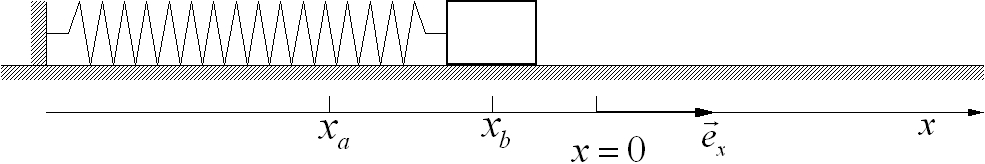
\includegraphics[width=0.85\textwidth ,angle=0]{elastische_energie}
	\end{image}
	
	\textsf{We willen de arbeid berekenen door de veerkracht geleverd op een massa bij de verplaatsing van een verlenging $x_a$ naar een verlenging $x_b$. Volgens de definitie wordt dit:}
	\begin{eqnarray*}
	W\,=\,\int_{x_a}^{x_b}F(x)~dx&=&\int_{x_a}^{x_b}-kx~dx\\
	&=&-k\left[\frac{x^2}{2}\right]_{x_a}^{x_b}\\
	&=&\frac{1}{2}k{x_a}^2-\frac{1}{2}k{x_b}^2
	\end{eqnarray*}
	\textsf{Indien het beginpunt $x_a$ verder uit de evenwichtspositie ligt dan het eindpunt $x_b$ is de geleverde arbeid positief.}}
	
	
	
	
\end{document}
